\documentclass[tikz,border=2pt]{standalone}
\usepackage{amsmath,amssymb}
\usepackage{tikz}
\usetikzlibrary{arrows.meta}

\begin{document}
% Chicken-egg: a Poisson number N of eggs, each hatching independently with probability p.
% The hatched and unhatched counts are independent Poisson variables.
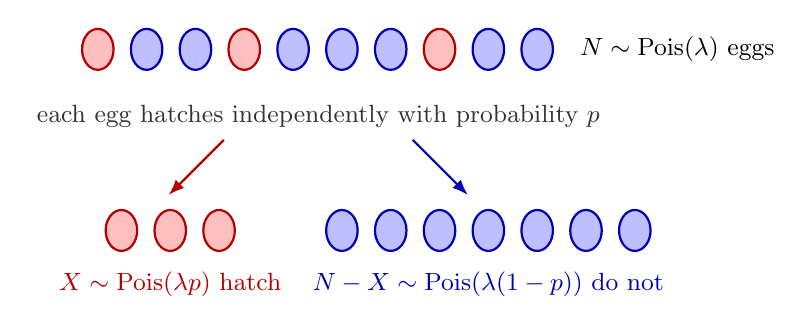
\begin{tikzpicture}[every node/.style={font=\small}, >={Latex[length=2mm]}]
	\foreach \x/\c in {0/red, 1/blue, 2/blue, 3/red, 4/blue, 5/blue, 6/blue, 7/red, 8/blue, 9/blue} {
		\draw[\c!70!black, fill=\c!25, thick] (0.62*\x,0) ellipse (0.2 and 0.26);
	}
	\node[anchor=west] at (6.0,0) {$N\sim\operatorname{Pois}(\lambda)$ eggs};
	\node[font=\small, gray!40!black] at (2.8,-0.85) {each egg hatches independently with probability $p$};
	\draw[->, thick, red!70!black] (1.6,-1.15) -- (0.9,-1.85);
	\draw[->, thick, blue!70!black] (4.0,-1.15) -- (4.7,-1.85);
	\foreach \x in {0,1,2} {
		\draw[red!70!black, fill=red!25, thick] (0.3+0.62*\x,-2.3) ellipse (0.2 and 0.26);
	}
	\foreach \x in {0,...,6} {
		\draw[blue!70!black, fill=blue!25, thick] (3.1+0.62*\x,-2.3) ellipse (0.2 and 0.26);
	}
	\node[red!70!black, anchor=north] at (0.92,-2.7) {$X\sim\operatorname{Pois}(\lambda p)$ hatch};
	\node[blue!70!black, anchor=north] at (4.96,-2.7) {$N-X\sim\operatorname{Pois}(\lambda(1-p))$ do not};
	
\end{tikzpicture}
\end{document}
